\documentclass[
	a4paper,
	oneside,
	BCOR = 10mm,
	DIV = 12,
	12pt,
	headings = normal,
]{scrartcl}

%%% Length calculations
\usepackage{calc}
%%%

%%% Support for color
\usepackage{xcolor}
\definecolor{lightblue}{HTML}{03A9F4}
\definecolor{red}{HTML}{F44336}
%%%

%%% Including graphics
\usepackage{graphicx}
%%%

%%% Font selection
\usepackage{fontspec}

\setromanfont{STIX Two Text}[
	SmallCapsFeatures = {LetterSpace = 8},
]

\setsansfont{IBM Plex Sans}[
	Scale = MatchUppercase,
]

\setmonofont{IBM Plex Mono}[
	Scale = MatchUppercase,
]
%%%

%%% Math typesetting
\usepackage{amsmath}

\usepackage{unicode-math}
\setmathfont{STIX Two Math}

\usepackage{IEEEtrantools}
%%%

%%% List settings
\usepackage{enumitem}
\setlist[enumerate]{
	label*      = {\arabic*.},
	leftmargin  = *,
	labelindent = \parindent,
	topsep      = 1\baselineskip,
	parsep      = 0\baselineskip,
	itemsep     = 1\baselineskip,
	noitemsep, % override itemsep
}

\setlist[itemize]{
	label*      = {—},
	leftmargin  = *,
	labelindent = \parindent,
	topsep      = 1\baselineskip,
	parsep      = 0\baselineskip,
	itemsep     = 1\baselineskip,
	noitemsep, % override itemsep
}

\setlist[description]{
	font        = {\rmfamily\upshape\bfseries},
	topsep      = 1\baselineskip,
	parsep      = 0\baselineskip,
	itemsep     = 0\baselineskip,
}

%%%

%%% Structural elements typesetting
\setkomafont{pagenumber}{\rmfamily\upshape}
\setkomafont{disposition}{\rmfamily\bfseries}

% Sectioning
\RedeclareSectionCommand[
	beforeskip = -1\baselineskip,
	afterskip  = 1\baselineskip,
	font       = {\normalsize\bfseries\scshape},
]{section}

\RedeclareSectionCommand[
	beforeskip = -1\baselineskip,
	afterskip  = 1\baselineskip,
	font       = {\normalsize\bfseries\itshape},
]{subsection}

\RedeclareSectionCommand[
	beforeskip = -1\baselineskip,
	afterskip  = 1\baselineskip,
	font       = {\normalsize\bfseries},
]{subsubsection}

\RedeclareSectionCommand[
	beforeskip = -1\baselineskip,
	afterskip  = -0.5em,
	font       = {\normalsize\mdseries\scshape\addfontfeatures{Letters = {UppercaseSmallCaps}}},
]{paragraph}
%%%

%%% Typographic enhancements
\usepackage{microtype}
%%%

%%% Language-specific settings
\usepackage{polyglossia}
\setmainlanguage{ukrainian}
\setotherlanguages{english}
%%%

%%% Captions
\usepackage{caption}
\usepackage{subcaption}

%\DeclareCaptionLabelFormat{closing}{#2)}
%\captionsetup[subtable]{labelformat = closing}

%\captionsetup[subfigure]{labelformat = closing}

\captionsetup[table]{
	aboveskip = 0\baselineskip,
	belowskip = 0\baselineskip,
}

\captionsetup[figure]{
	aboveskip = 1\baselineskip,
	belowskip = 0\baselineskip,
}

\captionsetup[subfigure]{
	labelformat = simple,
	labelformat = brace,
}
%%%

%%% Hyphenated ragged typesetting
\usepackage{ragged2e}
%%%

%%% Table typesetting
\usepackage{booktabs}
\usepackage{longtable}

\usepackage{multirow}

\usepackage{array}
\newcolumntype{v}[1]{>{\RaggedRight\arraybackslash\hspace{0pt}}p{#1}}
\newcolumntype{b}[1]{>{\Centering\arraybackslash\hspace{0pt}}p{#1}}
\newcolumntype{n}[1]{>{\RaggedLeft\arraybackslash\hspace{0pt}}p{#1}}
%%%

%%% Drawing
\usepackage{tikz}
\usepackage{tikzscale}
\usetikzlibrary{positioning}
\usetikzlibrary{arrows.meta} % Stealth arrow tips
%%%

%%% SI units typesetting
\usepackage{siunitx}
\sisetup{
	output-decimal-marker = {,},
	exponent-product      = {\cdot},
	inter-unit-product    = \ensuremath{{} \cdot {}},
	per-mode              = symbol,
}
%%%

%%% Framing code listings
\usepackage{tcolorbox}
\tcbuselibrary{breakable}
\tcbuselibrary{minted}
\tcbuselibrary{skins}

\newtcblisting[
	auto counter, 
	list inside, 
	number within = section,
]{listingpython}[3][]{%
	minted language = python,
	minted style    = bw,
	minted options  = {
		linenos,
		tabsize = 4,
		breaklines,
		% breakanywhere,
		fontsize = \footnotesize,
		autogobble
	},
	%
	% empty,
	sharp corners,
	colframe         = black,
	colback          = black!0,
	leftrule         = 0em,
	rightrule        = 0em,
	toprule          = 1pt, % orig = 0pt
	bottomrule       = 1pt, % orig = 0pt
	titlerule        = 0.5pt,
	colbacktitle     = black!0,
	coltitle         = black,
	toptitle         = 0.3em,
	bottomtitle      = 0.1em,
	borderline north = {1pt}{0pt}{black},
	borderline south = {1pt}{0pt}{black},
	before skip      = \intextsep,
	after  skip      = \intextsep,
	title            = {Лістинг \thetcbcounter: #2},
	list entry       = {\protect\numberline{\thetcbcounter}#2},
	left = 0em,
	right = 0em,
	%
	listing only,
	breakable,
	%
	label = {#3},
	%
	#1
}

\newtcbinputlisting[auto counter, list inside, number within = section]{\inputpython}[4][]{%
	minted language = python,
	minted style    = bw,
	minted options  = {
		linenos,
		tabsize = 4,
		breaklines,
		breakbytokenanywhere,
		fontsize = \footnotesize,
	},
	%
	% empty,
	sharp corners,
	colframe         = black,
	colback          = black!0,
	leftrule         = 0em,
	rightrule        = 0em,
	toprule          = 0pt, % orig = 0pt
	bottomrule       = 0pt, % orig = 0pt
	titlerule        = 0.5pt,
	colbacktitle     = black!0,
	coltitle         = black,
	toptitle         = 0.3em,
	bottomtitle      = 0.1em,
	borderline north = {1pt}{0pt}{black},
	borderline south = {1pt}{0pt}{black},
	before skip      = \intextsep,
	after  skip      = \intextsep,
	title            = {Лістинг \thetcbcounter: #3},
	list entry       = {\protect\numberline{\thetcbcounter}#3},
	left = 0em,
	right = 0em,
	%
	listing file={#2},
	listing only,
	breakable,
	%
	label = {#4},
	%
	#1
}

% Customize minted
\usepackage{minted}
\setmintedinline{
	style = bw,
	breaklines,
}

% Customize minted line numbers
\renewcommand{\theFancyVerbLine}{\ttfamily\scriptsize\arabic{FancyVerbLine}}

%%%

%%% Links and hyperreferences
\usepackage{hyperref}
\hypersetup{
	bookmarksnumbered = true,
	colorlinks      = false,
	linkbordercolor = red,
	urlbordercolor  = lightblue,
	pdfborderstyle  = {/S/U/W 1.5},
}
%%%

%%% Length adjustments
% Set baselineskip, default is 14.5 pt
\linespread{1.068966} % ~15.5 pt
\setlength{\emergencystretch}{2em}
\setlength{\parindent}{1.5em}
\newlength{\gridunitwidth}
\setlength{\gridunitwidth}{\textwidth / 12}
%%%

%%% Custom commands
\newcommand{\allcaps}[1]{{\addfontfeatures{LetterSpace = 8, Kerning = Off}#1}}
\newcommand{\filename}[1]{\texttt{#1}}
\newcommand{\progname}[1]{\texttt{#1}}
\newcommand{\modulename}[1]{\texttt{#1}}

\newcommand{\schel}[1]{\textit{#1}}
%%%

%%% Custom math commands
\newcommand{\longvar}[1]{\mathit{#1}}
%%%

\begin{document}

\begin{titlepage}
		\begin{center}
			Міністерство освіти і~науки України\\
			Національний авіаційний університет\\
			Навчально-науковий інститут комп'ютерних інформаційних технологій\\
			Кафедра комп'ютеризованих систем управління

			\vspace{\fill}
				Лабораторна робота №7\\
				з~дисципліни «Діагностика та~експлуатація комп'ютера»\\
				на~тему «Діагностика та~ремонт звукової карти»\\

			\vspace{\fill}

			\begin{flushright}
				Виконав:\\
				студент \allcaps{ННІКІТ}\\
				групи СП-325\\
				Клокун В.\,Д.\\
				Перевірила:\\
				Голего Н.\,М.
			\end{flushright}

			Київ 2019
		\end{center}
	\end{titlepage}

	\section{Мета роботи}
		Ознайомлення з~методами діагностики та~ремонту звуковоїкарти. 

	\section{Хід роботи}
		\subsection{Перевірка звукової карти за~допомогою програми~\textenglish{Sound Card Analyzer}}
			Перевіряємо звуковукарту за~допомогою програми~\textenglish{Sound Card Analyzer}. Для~цього запускаємо програму і~встановлюємо необхідні налаштування~(рис.~\ref{fig:sca}). 
			
			\begin{figure}[!htbp]
				\centering
				\begin{subfigure}[t]{\columnwidth / 2}
					\centering
					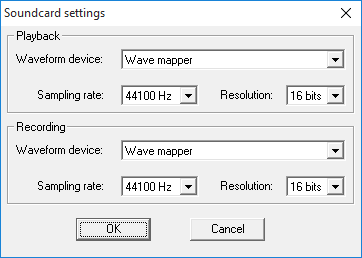
\includegraphics[height=8\baselineskip]{./assets/y03s02-pcdiag-lab-07-p00-01-sca-prerun.png}
					\caption{}
					\label{subfig:sca-prerun-01}
				\end{subfigure}%
				\begin{subfigure}[t]{\columnwidth / 2}
					\centering
					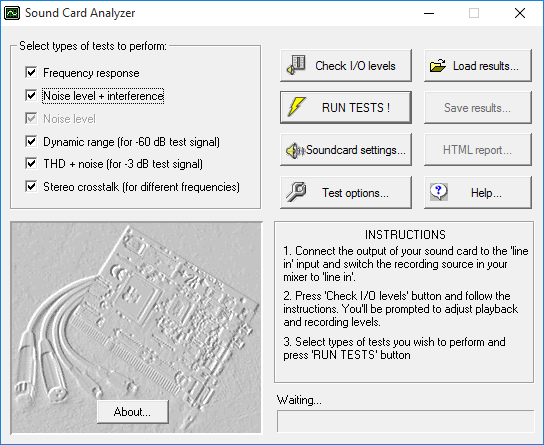
\includegraphics[height=10\baselineskip]{./assets/y03s02-pcdiag-lab-07-p00-02-sca-prerun.png}
					\caption{}
					\label{subfig:sca-prerun-02}
				\end{subfigure}
				\caption{Налаштування програми~\textenglish{Sound Card Analyzer}: \subref{subfig:sca-prerun-01}~— власне програми, \subref{subfig:sca-prerun-02}~— тестів}
				\label{fig:sca}
			\end{figure}

			Після встановлення налаштувань, запускаємо програму, натиснувши кнопку~«\textenglish{RUN TESTS!}», чекаємо, коли вона завершить виконання, та~спостерігаємо результат~(рис.~\ref{fig:sca-test}).

			\begin{figure}[!htbp]
				\centering
				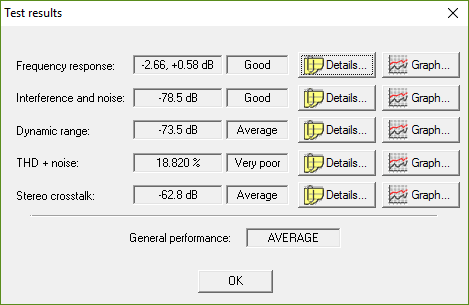
\includegraphics[height=8\baselineskip]{./assets/y03s02-pcdiag-lab-07-p01-01-test-res.png}
				\caption{Загальний результат тестування програмою~\textenglish{Sound Card Analyzer}}
				\label{fig:sca-test}
			\end{figure}

			Розглядаємо деталізацію тестів: «\textenglish{Frequency Response}»~(рис.~\ref{fig:sca-freq}), «\textenglish{Noise Level + Interference}»~(рис.~\ref{fig:sca-noise}), «\textenglish{Dynamic Range}»~(рис.~\ref{fig:sca-dynrange}), «\textenglish{THD + Noise}»~(рис.~\ref{fig:sca-thd}), «\textenglish{Stereo Crosstalk}»~(рис.~\ref{fig:sca-crosstalk}), .

			\begin{figure}[!htbp]
				\centering
				\begin{subfigure}[t]{\columnwidth / 2}
					\centering
					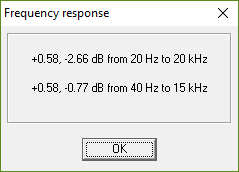
\includegraphics[height=08\baselineskip]{./assets/y03s02-pcdiag-lab-07-p02-01-freq.png}
					\caption{}
					\label{subfig:sca-freq}
				\end{subfigure}%
				\begin{subfigure}[t]{\columnwidth / 2}
					\centering
					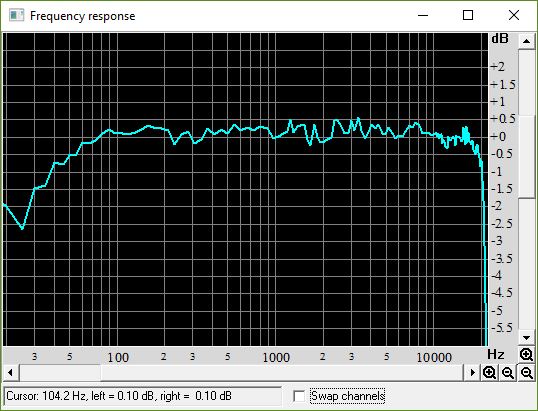
\includegraphics[height=08\baselineskip]{./assets/y03s02-pcdiag-lab-07-p02-02-freq-det.png}
					\caption{}
					\label{subfig:sca-freq-det}
				\end{subfigure}
				\caption{Результати тесту~«\textenglish{Frequency Response}»: \subref{subfig:sca-freq}~— стислі, \subref{subfig:sca-freq-det}~— розгорнуті}
				\label{fig:sca-freq}
			\end{figure}

			\begin{figure}[!htbp]
				\centering
				\begin{subfigure}[t]{\columnwidth / 2}
					\centering
					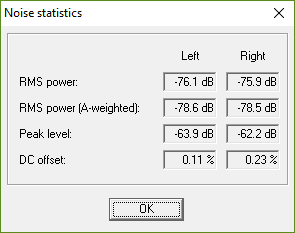
\includegraphics[height=08\baselineskip]{./assets/y03s02-pcdiag-lab-07-p03-01-noise.png}
					\caption{}
					\label{subfig:sca-noise}
				\end{subfigure}%
				\begin{subfigure}[t]{\columnwidth / 2}
					\centering
					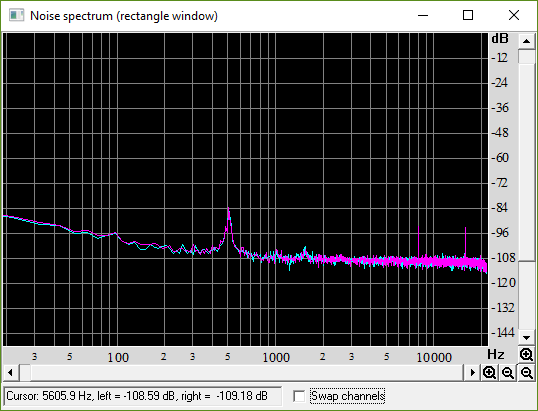
\includegraphics[height=08\baselineskip]{./assets/y03s02-pcdiag-lab-07-p03-02-noise-det.png}
					\caption{}
					\label{subfig:sca-noise-det}
				\end{subfigure}
				\caption{Результати тесту~«\textenglish{Noise Level + Interference}»: \subref{subfig:sca-noise}~— стислі, \subref{subfig:sca-noise-det}~— розгорнуті}
				\label{fig:sca-noise}
			\end{figure}

			\begin{figure}[!htbp]
				\centering
				\begin{subfigure}[t]{\columnwidth / 2}
					\centering
					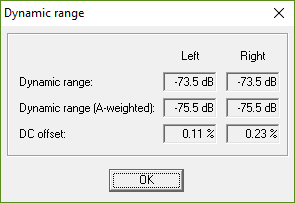
\includegraphics[height=08\baselineskip]{./assets/y03s02-pcdiag-lab-07-p04-01-dynrange.png}
					\caption{}
					\label{subfig:sca-dynrange}
				\end{subfigure}%
				\begin{subfigure}[t]{\columnwidth / 2}
					\centering
					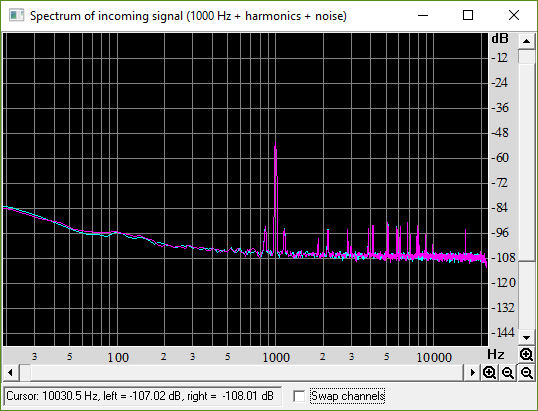
\includegraphics[height=08\baselineskip]{./assets/y03s02-pcdiag-lab-07-p04-02-dynrange-det.png}
					\caption{}
					\label{subfig:sca-dynrange-det}
				\end{subfigure}
				\caption{Результати тесту~«\textenglish{Dynamic Range}»: \subref{subfig:sca-dynrange}~— стислі, \subref{subfig:sca-dynrange-det}~— розгорнуті}
				\label{fig:sca-dynrange}
			\end{figure}
	
			\begin{figure}[!htbp]
				\centering
				\begin{subfigure}[t]{\columnwidth / 2}
					\centering
					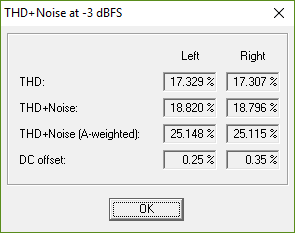
\includegraphics[height=08\baselineskip]{./assets/y03s02-pcdiag-lab-07-p05-01-thd.png}
					\caption{}
					\label{subfig:sca-thd}
				\end{subfigure}%
				\begin{subfigure}[t]{\columnwidth / 2}
					\centering
					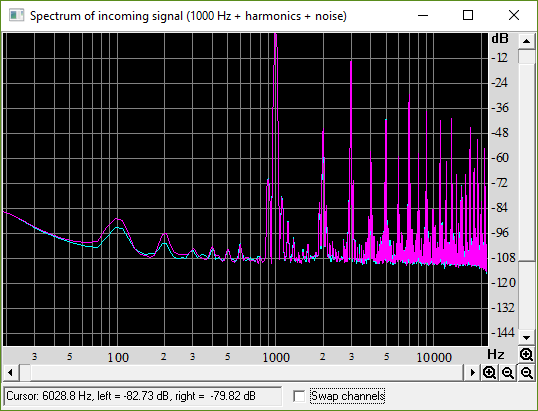
\includegraphics[height=08\baselineskip]{./assets/y03s02-pcdiag-lab-07-p05-02-thd-det.png}
					\caption{}
					\label{subfig:sca-thd-det}
				\end{subfigure}
				\caption{Результати тесту~«\textenglish{THD + Noise}»: \subref{subfig:sca-thd}~— стислі, \subref{subfig:sca-thd-det}~— розгорнуті}
				\label{fig:sca-thd}
			\end{figure}
	
			\begin{figure}[!htbp]
				\centering
				\begin{subfigure}[t]{\columnwidth / 2}
					\centering
					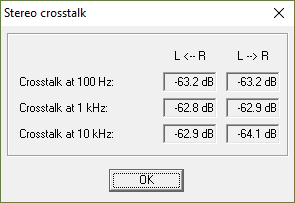
\includegraphics[height=08\baselineskip]{./assets/y03s02-pcdiag-lab-07-p06-01-crosstalk.png}
					\caption{}
					\label{subfig:sca-crosstalk}
				\end{subfigure}%
				\begin{subfigure}[t]{\columnwidth / 2}
					\centering
					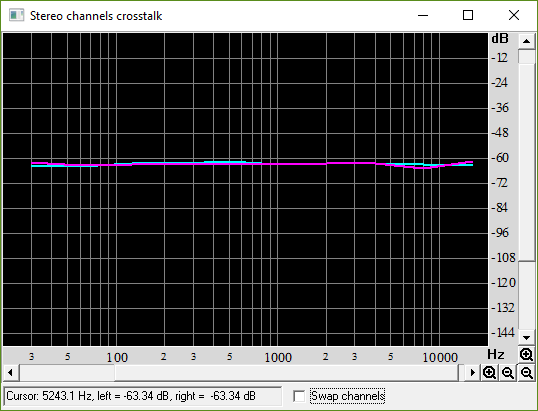
\includegraphics[height=08\baselineskip]{./assets/y03s02-pcdiag-lab-07-p06-02-crosstalk-det.png}
					\caption{}
					\label{subfig:sca-crosstalk-det}
				\end{subfigure}
				\caption{Результати тесту~«\textenglish{Stereo Crosstalk}»: \subref{subfig:sca-crosstalk}~— стислі, \subref{subfig:sca-crosstalk-det}~— розгорнуті}
				\label{fig:sca-crosstalk}
			\end{figure}

			В~результаті проходження тесту отримали дані про~характеристики звуку, який створює та~надсилає звукова карта, встановлена в~комп'ютері, у~вигляді числових даних та~графіків. 


	\section{Висновок}
		Виконуючи дану лабораторну роботу, ми~ознайомились з~методами діагностики та~ремонту звукової карти.

\end{document}

